% 
% Annual Cognitive Science Conference
% Sample LaTeX Paper -- Proceedings Format
% 

% Original : Ashwin Ram (ashwin@cc.gatech.edu)       04/01/1994
% Modified : Johanna Moore (jmoore@cs.pitt.edu)      03/17/1995
% Modified : David Noelle (noelle@ucsd.edu)          03/15/1996
% Modified : Pat Langley (langley@cs.stanford.edu)   01/26/1997
% Latex2e corrections by Ramin Charles Nakisa        01/28/1997 
% Modified : Tina Eliassi-Rad (eliassi@cs.wisc.edu)  01/31/1998
% Modified : Trisha Yannuzzi (trisha@ircs.upenn.edu) 12/28/1999 (in process)
% Modified : Mary Ellen Foster (M.E.Foster@ed.ac.uk) 12/11/2000
% Modified : Ken Forbus                              01/23/2004
% Modified : Eli M. Silk (esilk@pitt.edu)            05/24/2005
% Modified : Niels Taatgen (taatgen@cmu.edu)         10/24/2006
% Modified : David Noelle (dnoelle@ucmerced.edu)     11/19/2014

%% Change "letterpaper" in the following line to "a4paper" if you must.

\documentclass[10pt,letterpaper]{article}

\usepackage{cogsci}
\usepackage{pslatex}
\usepackage{apacite}
\usepackage{amsmath,amssymb}
\usepackage{graphicx}
\usepackage{color}
%\usepackage{hyperref}
\newcommand{\url}[1]{$#1$}


\definecolor{Red}{RGB}{255,0,0}
\newcommand{\red}[1]{\textcolor{Red}{#1}}

\newcommand{\subsubsubsection}[1]{{\em #1}}
\newcommand{\eref}[1]{(\ref{#1})}
\newcommand{\tableref}[1]{Table \ref{#1}}
\newcommand{\figref}[1]{Figure \ref{#1}}
\newcommand{\appref}[1]{Appendix \ref{#1}}
\newcommand{\sectionref}[1]{Section \ref{#1}}

\title{Wonky worlds: Listeners reconsider common ground when utterances are odd}
%Non-sinking marbles are wonky: defeasible world knowledge in language interpretation}

 
\author{{\large \bf Judith Degen, Michael H.~Tessler, Noah D.~Goodman} \\
  \{jdegen,mtessler,ngoodman\}@stanford.edu\\
  Department of Psychology, 450 Serra Mall \\
  Stanford, CA 94305 USA}

% ggplot colors: "#F8766D", "#A3A500", "#00BF7D", "#E76BF3", "#00B0F6"

\begin{document}

\maketitle


\begin{abstract}
World knowledge enters pragmatic utterance interpretation in complex ways. Sometimes, a speaker's utterance suggests that listeners should disregard their world knowledge, yet current models of pragmatic interpretation either disregard the role of world knowledge or overestimate its role in interpretation. Here we provide an extension to the Rational Speech Act model of scalar implicature that captures whether listeners believe they are in an abnormal--or `wonky'--world after observing a speaker's utterance, in which case they downweight their prior beliefs in the computation of speaker meaning. We show in four experiments that a) listeners have varying prior beliefs about the probability of various objects exhibiting an effect (e.g., marbles sinking), b) these beliefs influence listeners' expectations about how many objects will show the effect after observing an utterance (like \emph{Some of the marbles sank}), c) these beliefs influence scalar implicature strength, and d) listeners' world wonkiness judgments are affected by the surprisal of the observed utterance under their prior beliefs. The extended model is the first quantitative model that accounts for how rational listeners should integrate world knowledge in pragmatic utterance interpretation, and provides a close match to the empirically obtained data.

\textbf{Keywords:} 
scalar implicature; world knowledge; prior beliefs; experimental pragmatics; computational pragmatics
\end{abstract}

How often do you think marbles would sink in water? Probably extremely often, if not always. Now imagine reading \emph{Max threw fifteen of his favorite marbles in the water. Some of them sank.} Have you begun to reconsider your assumptions? Perhaps you now suspect that these marbles are in fact made of plastic or the water is covered with thick algae? That is, that they are not just normal marbles in normal water. Here we explore how prior world knowledge enters into pragmatic utterance interpretation, and how this world knowledge is defeasible: some utterances lead listeners to conclude that the world under discussion is abnormal and has appropriately different prior probabilities. We refer to such an abnormal world  as a \emph{wonky} world.

The Rational Speech Acts framework (RSA)  \cite{frank2012,goodman2013}, and related game-theoretic models \cite{franke2011}, treat communication as a signaling game \cite{lewis} between a speaker and a listener.
The listener reasons by Bayesian inference about what the world is like given that a speaker who produced the utterance is trying to be informative (with respect to a na\"ive listener). 
Variants of these models have successfully captured listeners' quantitative  behavior on a number of pragmatic inference tasks, including ad hoc Quantity implicature \red{ref}, M-implicature \red{ref}, scalar implicature \red{ref},  embedded scalar implicatures \red{ref}, and non-literal language \cite{kao2014}. 
A defining feature of Bayesian reasoning is that prior beliefs affect inferences that will be drawn. Bayesian models of language interpretation, accordingly, predict that prior beliefs about the world should affect the listener's interpretation of an utterance. 
%These models make clear predictions about how prior beliefs about states of the world should be integrated with listeners' expectations about utterances a speaker is likely to produce to communicate a particular state of the world. 
While this impact of prior knowledge has been noted, and included in models, it hasn't been systematically studied.

Generalizing our opening example, take the case of ``some of the X-s Y-ed'' (for category X and event Y). When the prior probability, $\theta_{X,Y}$, of an X Y-ing is not extreme, RSA leads to the standard scalar implicature: the posterior probability that all $15$ of the Xs Yed, after hearing the utterance, is much lower than its prior probability. This is because a rational speaker would have been expected to say the more informative ``all of the X-s Y-ed'' if it had been true.
As we will show in the next section, RSA makes two strong predictions about the effect of the prior: (1) As $\theta_{X,Y}$ approaches $1$ the interpretation probability that all X-s Y-ed approaches $1$, that is the scalar implicature disappears. 
This prediction follows because the extreme prior overwhelms the effect of the utterance.
(2) The posterior expectation of the number of X-s that Y-ed should be approximately the same as the prior expectation, when the number of tries is large (e.g.~15). 
This prediction follows from the weak semantics of ``some'' and the isolated effect of the alternative ``all'': because ``some of the X-s Y-ed'' only restricts the interpretation to be greater than zero and the scalar implicature resulting from alternative ``all of the X-s Y-ed'' can at the most rule out the all state, the prior will dominate the inference of exactly how many X-s Y-ed. 

However, intuition is at odds with these predictions: for example,  \citeA{geurts2010} has observed that for events with very high prior probability of occurrence (e.g.~marbles sinking), observing an utterance of \emph{Some of the marbles sank} leads to very strong implicatures, that is, the subjective probability that all of the marbles sank is intuitively close to 0. 
In Experiment 1 we collect prior probabilities for a variety of events and categories. In experiment 2a and 2b we collect posterior interpretations after hearing utterances such as ``some of the Xs Yed''. 
These experimental results confirm the intuition of relatively strong implicature---hence prediction (1) of RSA is incorrect---and show that the prior has a muted effect on posterior expectation---hence prediction (2) of RSA is incorrect.
Given the previous success of RSA models, this constitutes a striking puzzle. 
To address this puzzle we pursue the intuition raised at the very beginning of this paper: that sometimes, the speaker's utterance will lead the listener to infer that the world under discussion is wonky and she should therefore down-weight her prior beliefs in the computation of speaker meaning.
In Experiment 3 we explore participants' intuitions about whether the world is normal in the scenarios of Experiment 2.
We then introduce a variant of RSA, wRSA, in which the listener can revise her beliefs about the domain that the speaker intended. 
We show that this extension resolves the puzzle of the prior's muted effects, and predicts people's normalcy judgements.

% -illustrate why ``some'' is weird for high prior.
%-tie in to common ground (or wait for discussion?)

 

%\red{it's bold to make the intro so short.... i feel like a bit more is needed to set the stage for the paper. or possible the next section should just not be a separate section. at any rate, saying early the high level puzzle will help: Bayesian pragmatics sensitivity to the prior, we don't find this sensitivity. We suggest that this is because the (common ground) prior can be revised to accommodate otherwise unexplainable utterances.}




%World knowledge enters into the interpretation of utterances in complex ways. %For example, the plausibility of an NP as the subject of a sentence influences whether listeners are garden-pathed in cases like \textit{The horse raced past the barn fell} vs.~\textit{The landline buried in the sand exploded} \cite{bla}.
%While effects of world knowledge on syntactic processing are well-established, there is to date a surprising lack of systematic investigations into the effect of world knowledge in pragmatics. % -- this is especially surprising given that it has long been noted in the linguistics literature that pragmatics requires the integration of many different sources of linguistic and non-linguistic information. 
%Here, we provide a quantitative model of the effect of world knowledge  on  scalar implicatures, which are inferences that arise in cases of utterances like \textit{Some of the marbles sank}, %like (\ref{marbles}), where an utterance of (\ref{somemarbles}) 
%which typically gives rise to the inference that not all of the marbles sank.% in (\ref{simarbles}).
%
%\begin{exe}
%	\ex\label{marbles} 
%	\begin{xlist}
%		\ex\label{somemarbles} Some of the marbles sank.
%		\ex\label{simarbles} Not all of the marbles sank.
%	\end{xlist}
%\end{exe}


\section{Effect of the world prior in RSA}

The basic Rational Speech Acts model defines a pragmatic listener $P_{\textrm{listener}}(s|u)$, who reasons about a speaker $P_{\textrm{speaker}}(u|s)$, who in turn reasons about a literal listener $P_{\textrm{literal}}(s|u)$. Each listener does Bayesian inference about the world state, given either the literal truth of utterance $u$ or the speaker's choice of $u$; the speaker is a softmax-optimal decision maker, with the goal of being informative about the state $s$.
RSA is defined by:
\begin{eqnarray}
&&P_{\textrm{literal}}(s|u)\propto F_u(s) \cdot P(s)\\
&&P_{\textrm{speaker}}(u|s) \propto \mathrm{exp}({\lambda \ln P_{\textrm{literal}}(s|u))}\\
&&P_{\textrm{listener}}(s|u)\propto P_{\textrm{speaker}}(u|s)\cdot P(s)
\end{eqnarray}
Here $F_u: s \mapsto \{0,1\}$ is a truth-function specifying the meaning of each utterance.

For concreteness, assume that the set of states of the world is $S = \{s_0, s_1, s_2, \dots, s_{15}\}$, where the subscript indicates the number of objects (e.g., marbles) that exhibit a certain effect (e.g., sinking). 
Assume also that the set of utterances \emph{All/None/Some of the marbles sank} is denoted $U = \{u_{\textrm{all}}, u_{\textrm{none}}, u_{\textrm{some}}\}$ and each has it's usual literal meaning: 
$F_{u_{\textrm{none}}}(s) {=} \delta_{s=0}$,  
$F_{u_{\textrm{some}}}(s) {=} \delta_{s>0}$, 
$F_{u_{\textrm{all}}}(s) {=} \delta_{s=15}$.
Let us imagine that the prior is binomial with single event probability $\theta$: $P(s)=\text{Binomial}(s|\theta)$.

In Figure \ref{rss-basic} we show the predictions of RSA as $\theta$ varies. \red{put in figure showing the basic RSA predictions for allstate $P(s_{15}|u_{some})$ and expectation. this figure could also have wRSA predictions for later reference.} We see that the prior has a strong effect, which can be summarized by the two predictions described above. We next turn to an empirical test of these predictions, or rather, of the intuition that they may be incorrect.

%\section{Models of utterance interpretation}
%
%
%Recent Bayesian Rational Speech Act (RSA)  \cite{frank2012} and game-theoretic \cite{franke2011} models that treat communication as a signaling game \cite{lewis} between a speaker and a listener have successfully captured listeners' quantitative  behavior on a number of pragmatic inference tasks, including ad hoc Quantity implicature \red{ref}, M-implicature \red{ref}, scalar implicature \red{ref}, and embedded scalar implicatures \red{ref}. In these models, the listener reasons about likely utterances a speaker will produce who is trying to be informative with respect to a na\"ive listener. These models make clear predictions about how prior beliefs about states of the world should be integrated with listeners' expectations about utterances a speaker is likely to produce to communicate a particular state of the world. 
%
%\red{i think we should hold the math for the model section. it doesn't really add much here... without it, this section can be folded nicely into the introduction.}
%
%For concreteness, assume that $S = \{s_0, s_1, s_2, \dots, s_{15}\}$ is the set of states of the world, where the subscript indicates the number of objects (e.g., marbles) that exhibit a certain effect (e.g., sinking). Assume further that $U = \{u_{\textrm{all}}, u_{\textrm{none}}, u_{\textrm{some}}\}$, the set of utterances \emph{All/None/Some of the marbles sank}. The speaker chooses an utterance to convey $s$ proportional to the soft-max expected utility of producing $u$ to communicate $s$, where utility is determined by how uncertain a listener remains: \red{what's the expectation doing?}
%
%\begin{equation}
%P_{\textrm{speaker}}(u|s) \propto \mathrm{exp}({\lambda \mathbb{E} (\ln P_{\textrm{lex}}(s|u))})
%\end{equation}
%
%where $P_{\textrm{lex}}(s|u)$ is the literal interpretation probability resulting from each utterance's truth-functional meaning: $F_u: s \mapsto \{0,1\}$. \red{need to spell out lit listener since the prior enters there too} The listener's task is to infer a distribution over $S$, given an utterance $u$ produced by the above defined informative speaker. %$p(s|u)$, that is, the probability of the state of the world the speaker intended to communicate (e.g., how many friends came to a party), given that the speaker produced $u$ (e.g., \emph{some of my friends came to the party}). 
%By Bayes' rule: 
%\begin{equation}
%P_{\textrm{listener}}(s|u)\propto P_{\textrm{speaker}}(u|s)\cdot P(s)
%\end{equation}
%That is, the inferred listener probabilities are proportional to the product of both the speaker's utterance probabilities and the listener's prior beliefs in different numbers of marbles sinking. Using a uniform prior over the state space, this model has been very successful at capturing \emph{scalar implicatures} \cite{grice1975}. These are inferences that arise in cases of utterances like \textit{Some of the marbles sank}, which typically give rise to the inference that not all of the marbles sank. Scalar implicatures fall out of the fact that the speaker probability of producing $u_{\textrm{some}}$ in $s_{15}$ is low (because there is an alternative utterance $u_{\textrm{all}}$ which has a higher probability of being used for $s_{15}$ because it is more informative about that state). However, the role of prior beliefs in RSA models remains under-explored, both with respect to scalar implicature computation as well as with respect to utterance interpretation more generally.
%
%
%%One important consequence of the standard RSA model is that the listener's prior beliefs will not affect the interpretation of $u$ very strongly, if at all,  where the semantics of $u$ is highly constraining, that is, where  $P_{\textrm{lex}}(s|u)$ is very peaked. For example, an utterance of \emph{All of the marbles sank} is highly constraining because all of the probability mass ends up on $s_{15}$ by virtue of the semantics of $u_{\textrm{all}}$ alone, regardless of how likely the listener believes marbles sink a priori.\footnote{We ignore hyperbolic interpretations of universal quantifiers here.} 
%
%One important consequence of the standard RSA model is that where the semantics of $u$ is weak---that is, where $F_u$ accepts many states---prior beliefs are predicted to have a large effect on the resulting listener belief distribution. For example, an utterance of \emph{Some of the marbles sank}, produced in a situation in which any of 0 - 15 of 15 contextually established marbles could have sunk, semantically only restricts the state space by one state (that in which 0 marbles sank). In this case, listeners' prior beliefs about sinking marbles will have a large effect on their posterior belief distribution. If the listener believes that marbles rarely sink, the utterance will be interpreted as conveying that fewer marbles sank than if the listener believes marbles almost always sink. The predictions this model makes for the interpretation of $u_{\textrm{some}}$ -- both for $P_{\textrm{listener}}(s_{15}|u_{\textrm{some}})$ and for the expected value of $P_{\textrm{listener}}(s|u_{\textrm{some}})$ as a function of $P(s_{15})$ and the expected value of $P(s)$, respectively  -- are shown in \figref{fig:rrsaexppredictions}. RSA predicts that the probability of the state in which all objects exhibit a certain effect increases with increasing $P(s_{15})$, such that for $P(s_{15})$ close to 1, $P_{\textrm{listener}}(s_{15}|u_{\textrm{some}})$ approaches 1. Relatedly, with increasing expected value of the prior belief distribution $P(s)$, so is the expected value of the posterior belief distribution predicted to increase, approaching 1). \red{hmm... i think we either need to focus on the allstate probs for this motivation, or already point to the data from expt 1.}
%
%However, intuition is at odds with this prediction: for example,  \citeA{geurts2010} has observed that for events with very high prior probability of occurrence (e.g.~marbles sinking), observing an utterance of \emph{Some of the marbles sank} leads to very strong implicatures, that is, the subjective probability  that not all of the marbles sank is intuitively close to 0. Given the previous success of RSA models, this constitutes a striking puzzle, and one we set out to solve here. In doing so, we pursue the intuition raised at the very beginning of this paper: that sometimes, the speaker's utterance will lead the listener to infer that the world under discussion is wonky and she should therefore down-weight her prior beliefs in the computation of speaker meaning.
%
%
%Our contribution is two-fold: first, we collect empirical estimates of $P(s)$ and $P_{\textrm{listener}}(s|u)$ to investigate the empirical effect of listeners' prior beliefs on interpretation. Second, we extend the RSA model to incorporate a free variable $\theta_{\textrm{wonky}}$ that captures the extent to which the listener believes the described event is wonky  and she should thus discount her prior beliefs when interpreting $u$. We refer to this model as \emph{wonky RSA (wRSA)} in contrast to \emph{regular RSA (rRSA)}. Wonkiness inferences in wRSA are triggered by the surprisal of a produced utterance $u$, given listeners' prior beliefs, capturing that listeners expect speakers' utterances to be both truthful and informative with respect to prior beliefs. To the extent that they are not, listeners will have to either infer that the speaker is being uncooperative, or else assume that they may need to revise their beliefs about the world. Here we pursue the latter possibility.
%
%This paper is structured as follows. We first report the results of three experiments (1, 2a, 2b) that show that while there is an effect of the prior on listeners' interpretations of sentences like \emph{Some of the marbles sank}, this effect is much smaller than predicted by rRSA. Exp.~3 provides evidence that listeners' beliefs about object or event wonkiness are indeed influenced by the surprisal of the utterance. Finally, we present wRSA as an extension of rRSA that incorporates the idea of backing off to alternate prior beliefs if the observed utterance suggests a wonky world. This model provides a much better fit to the empirical data from Exps.~2a and 2b than rRSA, and also provides a good fit to the wonkiness ratings obtained in Exp.~3.

\begin{figure}
	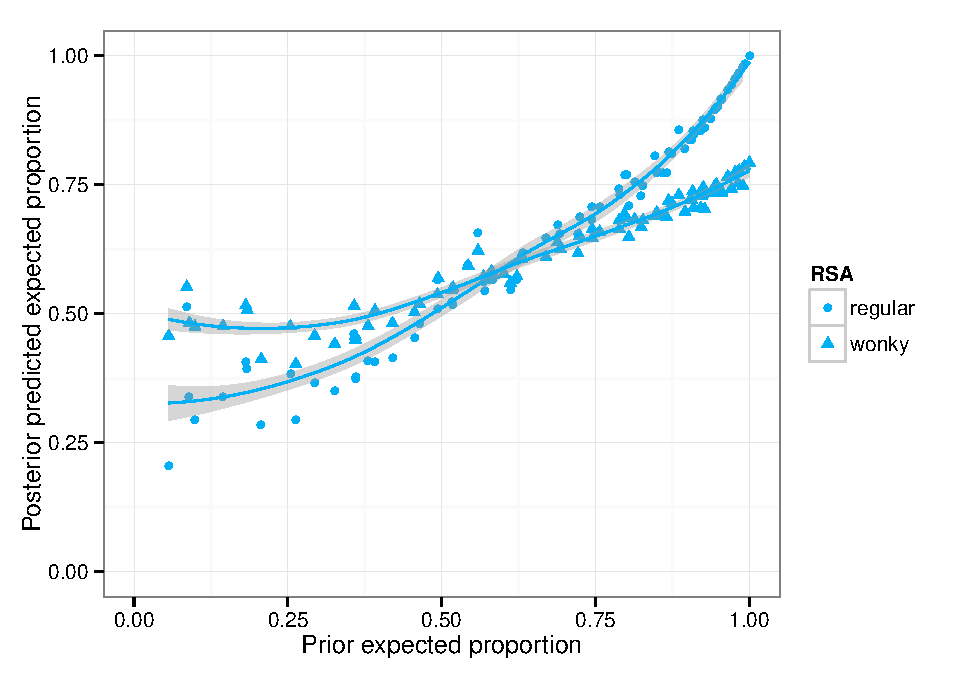
\includegraphics[width=.5\textwidth]{pics/model-expectations-uniform-regular}
	\caption{For each item, rRSA and wRSA model predicted mean empirical proportion of affected objects after observing \emph{Some of the X Yed}, as a function of prior mean proportion of affected objects.}
	\label{fig:rrsaexppredictions}	
\end{figure}

%\red{Include also plot of all-state probability: posterior empirical and predicted probability (rRSA, wRSA) as a function of prior all-state probability, for the SI people}




\section{Experiment 1} 

Exp.~1 measured participants' prior beliefs about how many times different objects would exhibit a certain effect (e.g., how many marbles sink), $P(s)$.

\subsection{Method}

\subsubsection{Participants}
We recruited 60 participants over Amazon's crowd-sourcing platform Mechanical Turk.

\subsubsection{Procedure and materials}

On each trial,\footnote{This experiment can be viewed at \url{https://www.stanford.edu/~jdegen/12_sinking-marbles-prior15/sinking-marbles-prior.html}} participants read a description of an event like \textit{John threw 15 marbles into a pool.} They were then asked to provide a judgment of an effect, e.g.~\textit{How many of the marbles do you think sank?}, on a sliding scale from 0 to 15. Judgments were obtained for 90 items, of which each participant saw a random selection of 30 items.
\red{should be more specific about the materials... each item had a similar form, with action, category, and outcome differing? say that we constructed them to cover the range of probabilities as much as possible.}

\subsection{Results}

Data from one participant, who gave only one response throughout the experiment, were excluded. Each item received between 12 and 29 ratings. Distributions of ratings for each item were smoothed using nonparametric density estimation for ordinal categorical variables \cite{liracine2003} using the \verb|np| package in R \cite{hayfield2013} \red{see hayfield 2013 np package specification for li and racine ref --- or laplace if that's what we use.}.

\red{say that we succeed in getting items that cover the probability range -- also maybe indicate how close the distributions are to binomial?}

\section{Experiment 2a}  
\red{if we end up tight on space, the expt 2a and 2b sections can be combined.}

\red{i think the current 2b should go first, since it uses the same DM as expt 1....}

Exp.~2a measured participants' posterior beliefs in different objects exhibiting a certain effect (e.g., marbles sinking), after observing an utterance, $p(s|u)$. 

\subsubsection{Participants}
We recruited 120 participants over Amazon�s crowd-sourcing platform Mechanical Turk.

\subsubsection{Procedure and materials}\footnote{This experiment can be viewed at \url{https://web.stanford.edu/~jdegen/sinking-marbles-nullutterance/sinking-marbles-nullutterance.html}}

Participants read the same descriptions as in Exp.~1. They additionally saw an utterance produced by a knowledgeable speaker about the event, e.g.~\textit{John, who observed what happened, said: ``Some of the marbles sank''}, and were asked to rate on sliding scales with endpoints labeled ``very unlikely'' and ``very likely'', how likely they thought 0\%, 1-50\%, 51-99\%, or 100\% of the marbles sank.


 Each participant saw 10 ``some'' trials and 20 fillers, of which 10 contained the quantifiers ``all'' or ``none'', and the rest were utterances that did not address the number of objects that displayed the effect, e.g.~\textit{What a stupid thing to do.} The utterances were randomly paired with 30 random items for each participant.
 
 
 \subsubsection{Results}
 \red{XXX question}

 $p(s_{\forall}|u_{\textrm{some}})$ increased with increasing \red{talk about both $p(s_{\forall}$ and the prior expectation of the distribution?} $p(s_{\forall}$) ($\beta$=.1, $SE$=.01, $t$=6.9, $p$$<$.0001); however, mean $p(s_{\forall}|u_{\textrm{some}})$ was never higher than .26, suggesting that a) participants drew strong implicatures in this paradigm and b) the effect of $P(s)$ is much smaller than predicted by rRSA.

\section{Experiment 2b}  

Exp.~2b replicates the effect of the prior on participants' posterior estimates of different objects exhibiting a certain effect (e.g., marbles sinking) using a different dependent measure. 

\subsubsection{Participants}
We recruited 120 participants over Amazon�s crowd-sourcing platform Mechanical Turk.

\subsubsection{Procedure and materials}\footnote{This experiment can be viewed at \url{https://www.stanford.edu/~jdegen/13_sinking-marbles-priordv-15/sinking-marbles.html}}

The procedure and materials were identical to those of Exp.~2a with the exception of the dependent measure. Rather than providing point estimates of the probability of different numbers of objects sinking, participants performed the task from Exp.~1, i.e., they were asked to provide a judgment of an effect, e.g.~\textit{How many of the marbles do you think sank?}, on a sliding scale from 0 to 15.
 
 \subsubsection{Results and discussion}
 \red{XXX question}

The mean number of objects judged to exhibit the effect increased with increasing expectation of the prior distribution ($\beta$=.18, $SE$=.02, $t$=7.4, $p$$<$.0001, see also \figref{fig:meanresponses}), replicating the effect observed in Exp.~2a. Again, the effect of the prior was much smaller than predicted by rRSA and resulted in mean proportions of affected objects between 30\% and 65\%, where rRSA predicts a range from \red{XXX} to \red{XXX} for these items.

\red{need to discuss fillers, and that this means the muted effect of prior is not because Ss are insensitive to it.}

\begin{figure}
	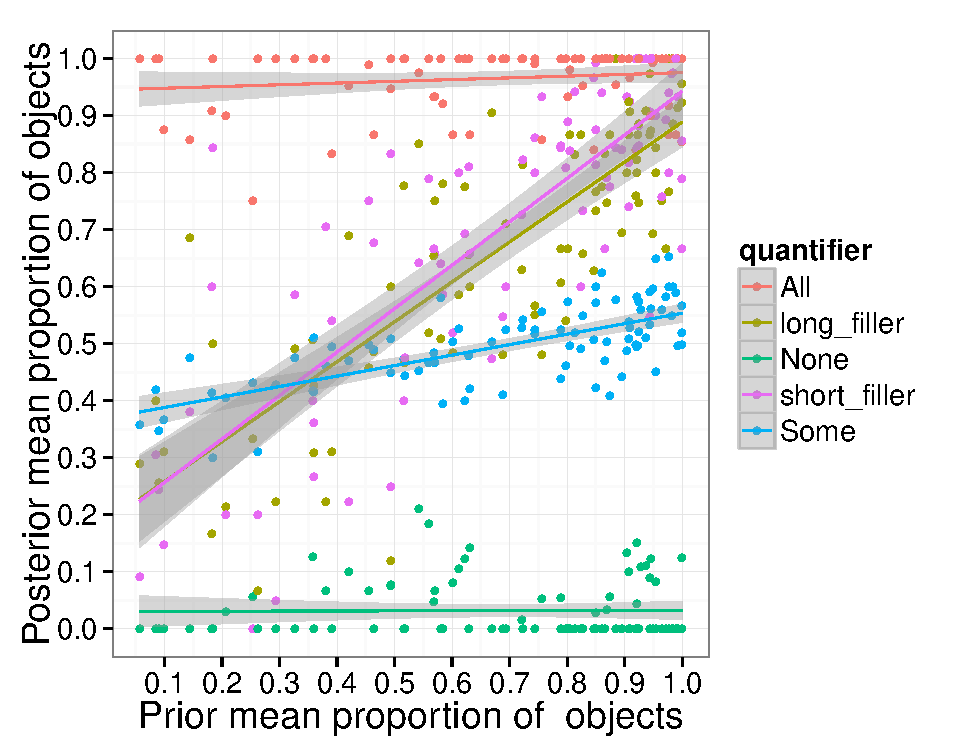
\includegraphics[width=.5\textwidth]{pics/meanresponses}
	\caption{For each item, mean empirical proportion of affected objects after observing an utterance, as a function of prior mean proportion, for different quantifiers and filler conditions. \red{two panels, one for 2a and one for 2b?}}
	\label{fig:meanresponses}	
\end{figure}

Exps.~2a and 2b demonstrate that there is an effect of listeners' prior beliefs on the interpretation of utterances with \emph{some}. However, this effect is quantitatively much smaller than predicted by rRSA, and qualitatively does not show the critical limit effect (converging to the upper-right corner as seen in Fig.~\ref{fig:rrsaexppredictions}).
\red{earlier be clear about the prediction that as prior goes to one allprob and expectation should go to one. reference that qualitative prediction of RSA here and in 2a results.}

\red{Discussion of why; wonky world intuition}

\section{Experiment 3}

Exp.~3 measured participants' beliefs in world wonkiness after observing the scenarios and utterances from Exps.~2a and 2b.

\subsubsection{Participants}
We recruited 60 participants over Amazon's crowd-sourcing platform Mechanical Turk.

\subsubsection{Procedure and materials}\footnote{This experiment can be viewed at \url{https://web.stanford.edu/~jdegen/17_sinking-marbles-normal-sliders/sinking-marbles-normal.html}}

The procedure and materials were identical to those of Exps.~2a and 2b, with the exception of the dependent measure. Rather than providing estimates of what they believed the world was like, participants were asked to indicate how likely it was that the objects  (e.g., the marbles) involved in the scenario were normal objects, by adjusting a slider that ranged from \emph{definitely not normal} to \emph{definitely normal}.

\subsubsection{Results}

The extreme ends of the sliders were coded as 1 (\emph{definitely not normal}, i.e., wonky) and 0 (\emph{definitely normal}, i.e., not wonky). We interpret the slider values as probability of world wonkiness. Mean wonkiness probability ratings are shown in \figref{fig:wonkyratings}. For \emph{all} and \emph{none}, increasing prior expectation of objects exhibiting the effect resulted in a fairly linear decrease and increase in the probability of wonkiness, respectively. For \emph{some}, the pattern is somewhat more intricate: probability of wonkiness initially decreases sharply, but rises again in the upper range of the prior expected value. 

\begin{figure}
	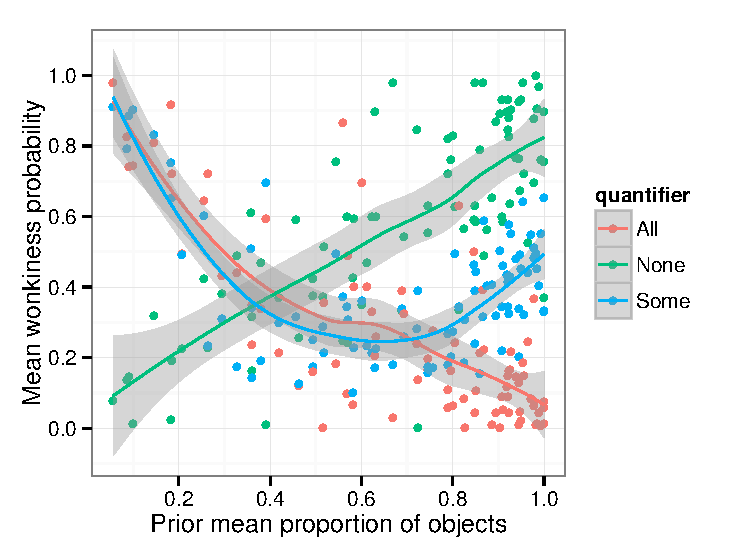
\includegraphics[width=.5\textwidth]{pics/probwonky-empirical}
	\caption{For each item, mean wonkiness probability after observing an utterance, as a function of expected prior proportion of affected objects, for different quantifiers.}
	\label{fig:wonkyratings}	
\end{figure}

\red{yay!! XXX}

\section{Model}


The wonky RSA model we propose for capturing the defeasibility of listeners' world knowledge is an extension of regular RSA: in wRSA, the listener infers the value of $\theta_{\textrm{wonky}}$ jointly with $s$. $\theta_{\textrm{wonky}}$ captures for each utterance and item, how likely the objects involved in the event (e.g., marbles) are in fact ``wonky'' (in which case the computation draws on a uniform prior, i.e.~disregards prior beliefs) or not (in which case the model draws on the smoothed empirical prior distribution for that item, obtained in Exp.~1). The resulting $p(s|u)$ is a mixture of computations based on the uniform and empirical prior, with mixture parameter $\theta_{\textrm{wonky}}$. The inferred value of $\theta_{\textrm{wonky}}$ itself depends on $p(u|s)$: the more surprising a particular utterance is given prior beliefs, the higher the probability of $\theta_{\textrm{wonky}}$.


%This `lifted variable' that can be conceived of as analogous to the lifted variable over lexica that is at the core of recent lexical uncertainty models of word learning \red{ref}, M-implicature, and embedded scalar implicature \cite{bergen2014}. The difference is that, rather than having uncertainty about the lexicon the listener believes the speaker to be employing, the listener has uncertainty about the speaker's prior beliefs. In particular, the speaker uses either the empirical prior (obtained in Exp.~1) or an alternative prior \red{DESCRIBE}. The pragmatic listener 


\red{NDG: note to self -- difference between revising own beliefs and revising common ground....}


\section{Model evaluation}

\begin{figure}

	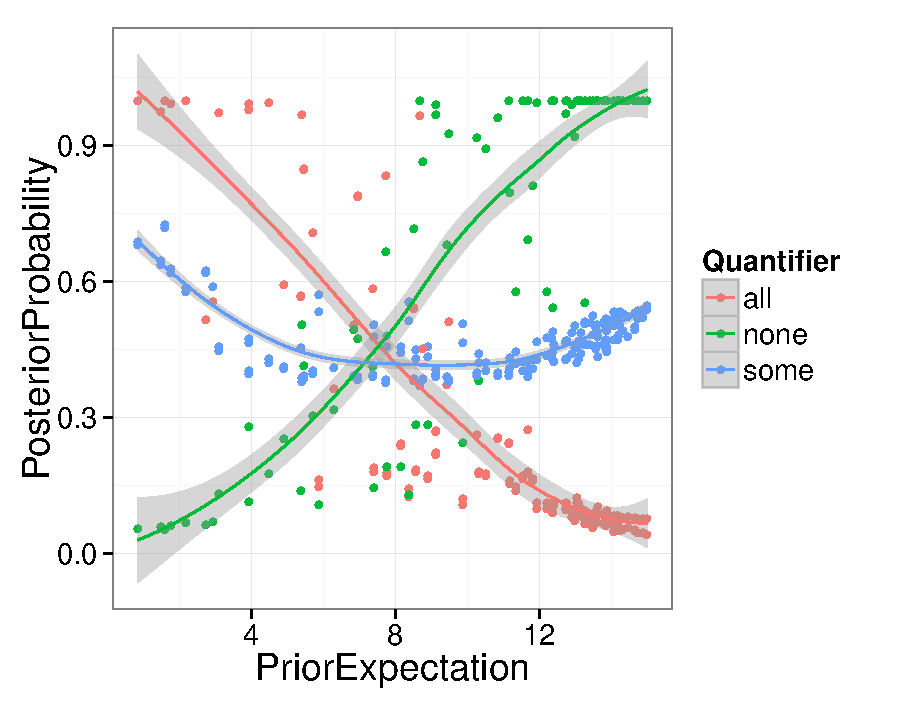
\includegraphics[width=.5\textwidth]{pics/proportionwonky-model}
	\caption{\red{For each item, predicted proportion of 'wonky' ratings after observing an utterance, as a function of prior mean proportion, for different quantifiers.}}
	\label{fig:wonkymodel}	
\end{figure}

\red{From the abstract: Comparing the fit of rRSA and wRSA model predictions to the posterior state estimates from Exp.~2 yields a much better fit for wRSA. The better fit of wRSA suggests that listeners  use speakers' utterances as cues to how strongly to incorporate world knowledge. wRSA also provided a better fit than a model which used only a uniform prior, confirming that listeners do make use of world knowledge in a systematic way in the computation of scalar implicature.}


\red{it's possible we'd get less noise form some more stable estimator of prior. consider trying the plots with prior mode and median as x-axis.... or inferred binomial prob fit to each prior, if the fits are at all decent.}


\section{Discussion and conclusion}

\begin{itemize}

	\item what is wonky?
	\item other ways of asking about wonkiness
	\item what's the right prior to back off to?
	\item revising private beliefs vs revising common ground.
	\item connection to presupposition (cf stalnaker), and other phenomena
	\item implication for experiments on language understanding

\end{itemize}



\bibliographystyle{apacite}

\setlength{\bibleftmargin}{.125in}
\setlength{\bibindent}{-\bibleftmargin}

\bibliography{bibs}


\end{document}
